% File example.tex
% Contact: simonnet@ecole.ensicaen.fr
%
% version 1.0 (July 24, 2009)
% version 1.1 (September 3, 2009)
% add using of the optional command: \secondauthoraddr



\documentclass[10pt]{article}

% File icdp2009.sty
% Preamble that you have to include to use the template  

% July 24, 2009
% Contact: simonnet@ecole.ensicaen.fr


\usepackage[a4paper,textwidth=18cm,textheight=24cm,top=2.85cm, bottom=2.85cm, left=1.5cm, right=1.5cm]{geometry}

\usepackage{template/icdp2009}

% left justified caption
\makeatletter
\long\def\@makecaption#1#2{%
\vskip\abovecaptionskip
\sbox\@tempboxa{#1. #2}%
\ifdim \wd\@tempboxa >\hsize
#1. #2\par
\else
\global \@minipagefalse
\hb@xt@\hsize{\box\@tempboxa\hfil}%
\fi
\vskip\belowcaptionskip}
\makeatother




%other package
\usepackage{amsmath}

% vectorial font
\usepackage{lmodern}

\usepackage{graphicx}
\usepackage{times}


\begin{document}
\noindent

\bibliographystyle{plain}

\title{Naive Bayes Classifier\\Assignment 1 of Machine Learning I, 2021/2022}

\authorname{Mura Alessio}
\authoraddr{DIBRIS - Dipartimento di Informatica, Bioingegneria, Robotica e Ingegneria dei Sistemi\\
Università Degli Studi di Genova}

% \secondauthoraddr{+Affiliation,Country and contact details }


\maketitle

% % \keywords
% % Maximum 5 keywords placed before the abstract.

% \abstract
% This is where the abstract should be placed. It should consist
% of one paragraph and a concise summary of the material
% discussed in the article below. It is preferable not to use
% footnotes in the abstract or the title. The acknowledgement
% for funding organisations etc. is placed in a separate section at
% the end of the text. We wish you success with the preparation
% of your manuscript.

\section{Introduction}
Naive Bayes is a statistical classification technique based on Bayes Theorem. It is one of the simplest supervised learning algorithms. Naive Bayes classifier is the fast, accurate and reliable algorithm. Naive Bayes classifiers have high accuracy and speed on large datasets.

\section{Theory of NBC}
\subsection{Mathematical theory}
Let’s call the input \textit{x} \textit{(observation)}. A Classification is a rule
\textit{y()} that, given an input, produces an output called \textit{t (class)}, so that:
\begin{equation}
    t = y(x) 
\end{equation}
In order to output the most appropriate class, the classifier choose the classification that has the minimum error probability. In particular, the NBC is based on a \textit{naive} assumption,
which basically is not correct but works just the same:
\begin{equation}
    P_r(x_1, ..., x_d | t_i) = P_r(x_1|t_i)P_r(x_2|t_i) ... P_r(x_d|t_i)
\end{equation}
The NBC classifier therefore pretends that input variables are
all independent of each other. \\\\
To select the best class we use a discriminant function \textit{$g_i(x)$}.
This function can be compute as follows:
\begin{equation}\label{e:barwq}\begin{split}
    g_i(x)& = P_r(t_i)[P_r(x_1|t_i)P_r(x_2|t_i) ... P_r(x_d|t_i)] = \\
   & = P_r(t_i) \prod_{j=1}^{d}P_r(x_j|t_d)
\end{split}\end{equation}

After computing every \textit{$g_i(x)$}, the classifier takes the one
that has the highest value, and classifies \textit{x} with \textit{t}.
\subsection{Training session}
During the training session the classifier acquires data
from the training set. In particular the NBC computes every
conditional probability, using this formula:

\begin{equation}
     P_r(x_j = v_k|t_i) = \frac{\text{number of $x_j = v_j$ in class $t_i$}}{\text{number of instance of $t_i$}}
\end{equation}
where $v_j$ is the possible value for the attribute \textit{j}.
\subsection{Improvements with Laplace Smoothing}
Using a small data set, some combinations that appear in
the test set were not encountered in the training set, so their
probability is assumed to be zero. When you multiply many
terms, just a zero sets the overall results to zero.\\\\
Generally speaking, some values of some attributes could
not appear in the training set, but are actually inside the
entire set. The classifier should know this information, and
the \textbf{Laplace Smoothing} comes in hand.\\\\With the Laplace smoothing, a \textit{trust factor} \textbf{a} is implemented
in the conditioned probability computation as follows:
\begin{equation}
     P_r(x_j = v_k|t_i) = \frac{\text{(number of $x_j = v_j$ in class $t_i$) + \textbf{a}}}{\text{(number of instance of $t_i$) + \textbf{a}v}}
\end{equation}
where \textit{v} is the number of possible values of the variable \textit{x}.
When $a < 1$ the classifier trusts his prior belief less than
the data, while with $a > 1$ the classifier trusts his prior belief
more than the data. Adding \textit{a} results in a probability that is
never equal to zero, even if the value does not appear in the
training set.


\section{THE ASSIGNMENT}
The given assignment consist of three tasks:
\begin{itemize}
 \item \textbf{Task 1}: Data pre-processing
 \item \textbf{Task 2}: Build a naive Bayes classifier
 \item \textbf{Task 3}: Improve the classifier with Laplace (additive) smoothing
 \end{itemize} 

\subsection{Task 1: Data pre-processing}
Our dataset is initially stored as .csv files. To import it in Python, it is required to use the function read-csv(), inside Pandas library, in order to store our data into a dataframe.
Usually attributes value should be converted
in positive integer values, in order to make them easier to
manipulate.
\newpage 
The used set is a Weather data set composed by:
\begin{itemize}
 \item  14 observations;
 \item 4 attributes (outlook, temperature, humidity, windy);
 \item 2 classes (play YES, play NO).
 \end{itemize}
The set is built in such a way that the first four columns
are the attributes, while the last column is the target of the
observation. In particular, outlook can assume three different
values \textit{(overcast, rainy or sunny)}, temperature can also assume
three different values \textit{(hot, mild or cool)}, humidity can assume
two values \textit{(high or normal)} and windy can assume two values
\textit{(true or false)}.

\subsection{Task 2: Build a naive Bayes classifier}
The naive Bayes classifier is divided in two sections: the
training section and the classification section. in order to compute the classification, we created a function: \textit{NaiveBayesClassifier()}.\\\\
Inside this function, we call other functions useful for the computation:
\begin{itemize}
    \item \textit{Likelihood()}
    \item \textit{FinalProbability()}
    \item \textit{Predictions()}
\end{itemize}
\subsubsection{Likelihood()}
In this function we pass three values: the \textbf{train-set}; a vector that counts the number of columns' unique values of the dataset (\textbf{v}) and our dataframe \textbf{df}.\\\\
This function is useful for computing the occurrences of \textit{Yes (value = 2)} and \textit{No (value = 1)} in the target column. In fact, the final result will be two different lists containing the occurrences for each of the four attributes (outlook, temperature, humidity, windy) depending on the value of the target column (yes or no).
\\\\ 
Moreover, inside this function it is called another function, \textit{LaplaceSmoothing()}, but this will be topic of discussion in subsection 3.3.
\subsubsection{FinalProbability()}
In this function, we  classified each observation that was inside the test set, according to the inferred rule
of maximizing the discriminant function $g_i(x)$ (equation 3).
\\\\
we also called a function, \textit{PriorProbability()}, in order to compute the prior probability of \textit{Yes} and \textit{No}.
\\\\
The function's outputs are two lists: \textbf{final-yes}, which contains the probability of \textit{yes} and \textbf{final-no}, which contains the probability of \textit{no}.

\subsubsection{Predictions()}
This function is quite simple: we compare the final probability of \textit{yes} and the final probability of \textit{no} in order to compute the prediction.
\\\\ 
If the probability of \textit{Yes} is greater than the probability of \textit{No} the prediction returns \textit{yes (value: 2)}; whereas if the probability of \textit{No} is greater than the probability of \textit{Yes} the prediction returns \textit{no (value: 1)}.


\subsection{Task 3: Improve the classifier with Laplace (additive) smoothing}
As seen in the equation 5, the \textbf{a} factor is inserted inside
the equation 4. The a factor is specified inside \textit{LaplaceSmoothing()} function. The classifier is just the same as before, but this time according with the theory explained in subsection 2.3.
\\\\ 
We chose to assign it the value of 0.85, in order to make the classifier trusts his prior belief less than
the data.

\section{RESULTS}

\begin{figure}[h] 
	\centering
	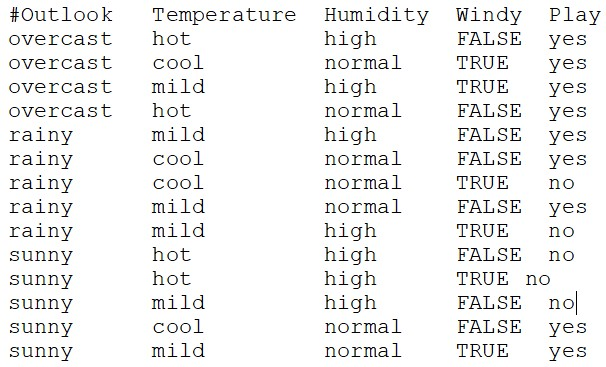
\includegraphics[width=0.9\columnwidth]{wheter.jpg} % Example image
	\caption{Wheather dataset}
\end{figure}
The figure 1 shows the dataset in which we computed our classification.

\begin{figure}[h] 
	\centering
	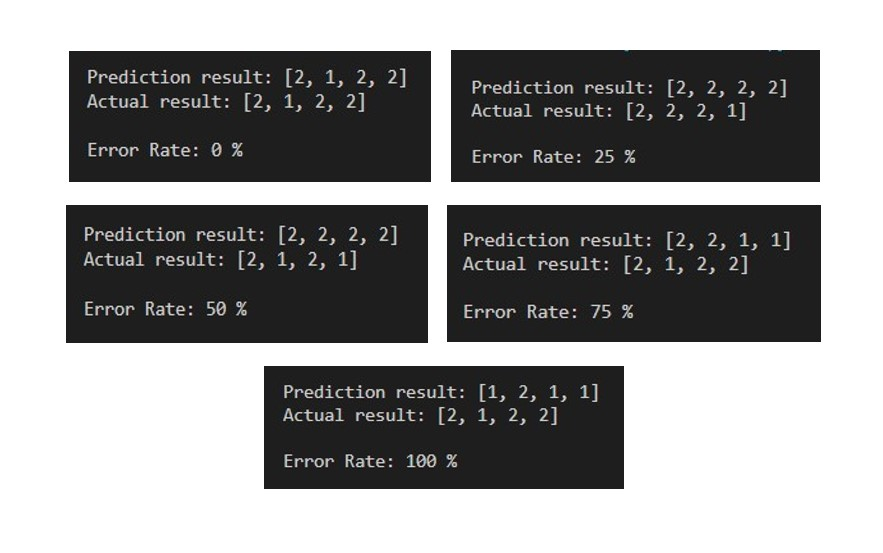
\includegraphics[width=1.0\columnwidth]{template/total.jpg} % Example image
 \caption{Results of classification}
\end{figure}
Each time we run our program, it will return on the console three parameters: the result of our prediction, the actual values and the error rate of our classification, as we can clearly see in figure 2.
\\\\ The error rate's value
is computed as the number of correct classification divided by
the number of observation. Notice that in this test, with only 4
observation inside the test set, the error rate can assume only
five fixed values:
\begin{itemize}
 \item  0 \% in case every classification is correct,
 \item 25 \% if there is only one wrong classification,
 \item 50 \% if there are two wrong classifications,
 \item 75 \% if there are three wrong classifications,
\item 100 \% in case every classification is incorrect.

 \end{itemize}

 \\\\
 All the classifications are executed with a training set made
of 10 observation and a test set made of 4 observation. With
two larger sets the Laplace could be more incisive in the
classification process.

\end{document}